\chapter{把方程放回重联层：Sweet--Parker、Hall层与电子层}
\label{hall:reconnection}
\section{为什么重联需要同时考虑入口与出口}
考虑稳态二维矩形扩散区，半长$L$，半厚$\delta$。上下两面入流，左右两面出流。若两侧对称，每单位$z$长度的质量通量是
\begin{equation}
2(2L)\rho_{\rm in}v_{\rm in}=2(2\delta)\rho_{\rm out}v_{\rm out}.
\end{equation}
每边都含两面和全长，约掉4，得到
\begin{equation}\rho_{\rm in}v_{\rm in}L=\rho_{\rm out}v_{\rm out}\delta.\end{equation}
若密度近似不变，再有$v_{\rm in}/v_{\rm out}=\delta/L$。因此长而窄的通道无法同时承载很大的入口质量通量和有限的出口速度；这不是电阻本身的结论，而是几何和质量守恒的约束。

磁张力将等离子体加速向外。按单位体积动量估计，惯性$\rho v_{\rm out}^2/L$与磁张力$B^2/(\mu_0L)$平衡，故
\begin{equation}v_{\rm out}\sim B/\sqrt{\mu_0\rho}=V_A.\end{equation}
这是假定下游背压、黏性、流剪切及其他能量损失没有强烈降低出流的量级关系，不是每个位置速度都恰好等于$V_A$。

\section{Sweet--Parker的三个条件如何一步步消元}
稳态二维Faraday定律要求$\partial_xE_z=\partial_yE_z=0$，故同一个$E_z$贯穿上游和扩散区。上游近理想，有$|E_z|\simeq v_{\rm in}B$；片心反向场很小，电阻模型给$|E_z|\simeq\eta|J_z|$。用$|J_z|\sim B/(\mu_0\delta)$，依次得到
\begin{align}
v_{\rm in}B&\sim\eta\frac{B}{\mu_0\delta},\\
v_{\rm in}&\sim\frac{D_\eta}{\delta}.
\end{align}
与连续性$v_{\rm in}\sim V_A\delta/L$相等：
\begin{align}
\frac{D_\eta}{\delta}&\sim\frac{V_A\delta}{L},\\
\delta^2&\sim\frac{D_\eta L}{V_A},\\
\boxed{\frac{\delta_{SP}}L\sim S_L^{-1/2}},\qquad
\boxed{\frac{v_{\rm in}}{V_A}\sim S_L^{-1/2}},\qquad S_L&=\frac{LV_A}{D_\eta}.
\end{align}
三个条件是质量通量、Alfvén量级出流和电场匹配。单独看欧姆定律无法决定$L$或$\delta$；把层长任意缩短，当然能得到更大速率，但那不是对层长选择的解释。

\worked{高密度教学例：一个较接近电阻MHD排序的情况}
用前章高密度例$L=10$ m、$V_A=3.4488\times10^4$ m/s、$D_\eta=51.386$ m$^2$/s，算得
\begin{align}
S_L&=\frac{10\times3.4488\times10^4}{51.386}=6.71\times10^3,\\
\delta_{SP}&=\frac{10}{\sqrt{6711.5}}=0.1221\,\mathrm m,\\
v_{\rm in}&=\frac{3.4488\times10^4}{\sqrt{6711.5}}=421\,\mathrm{m/s},\\
E_z&\sim v_{\rm in}B=21.0\,\mathrm{V/m}.
\end{align}
此时$d_i/\delta_{SP}=0.0590$、$\rho_i/\delta_{SP}=0.0529$、$\lambda_{\rm mfp,e}/\delta_{SP}=0.00597$。对于粗略的层结构，Hall和离子轨道尺度较小，碰撞局地性也更合理。它仍不是一个已证明稳定的实验解：大尺度稳定性、黏性和其他输运需要另查。

\worked{实验室教学例：全局MHD看似合理，内层却失败}
$S_L=3.7585\times10^4$、$\delta_{SP}=5.158$毫米、$v_{\rm in}=1.779$ km/s、$E_z=88.95$ V/m。核对电阻一侧：
\begin{equation}
J\sim\frac{0.05}{(1.25664\times10^{-6})(0.005158)}=7.71\times10^6\,\mathrm{A/m^2},
\quad \eta_DJ=88.95\,\mathrm{V/m}.
\end{equation}
数值匹配得很好，但$d_i/\delta_{SP}=13.96$、$\rho_i/\delta_{SP}=2.51$、$\lambda_{\rm mfp,e}/\delta_{SP}=158$。离子尺度比较已说明\textbf{我们解对了一个不适用的单流体经典电阻层模型}。平均自由程应与有关轨道方向、尤其平行方向的梯度尺度比较；此处与横向片厚的比值仅作警报，不能单独否定经典电阻闭合。代数自洽不等于物理自洽；下一步应检查双流体、压力张量和非局地闭合，而不是把这5毫米直接当预测。

\section{从一个不等式判断何时需要重新审查模型}
将$\delta_{SP}\lesssim d_i$代入上式：
\begin{align}
LS_L^{-1/2}&\lesssim d_i,\\
S_L^{1/2}&\gtrsim L/d_i,\\
\boxed{S_L\gtrsim(L/d_i)^2}.\label{hall:spthreshold}
\end{align}
这是反平行、该经典层宽估计下的\emph{自洽性警报}，不是普适Hall启动充分条件。系统是否到达该层宽、是否先发生撕裂/磁岛、是否强导场、边界怎样供磁、是否有迟滞，都能改变实际演化。\citep{Cassak2005,Ng2015}
\begin{figure}[htbp]\centering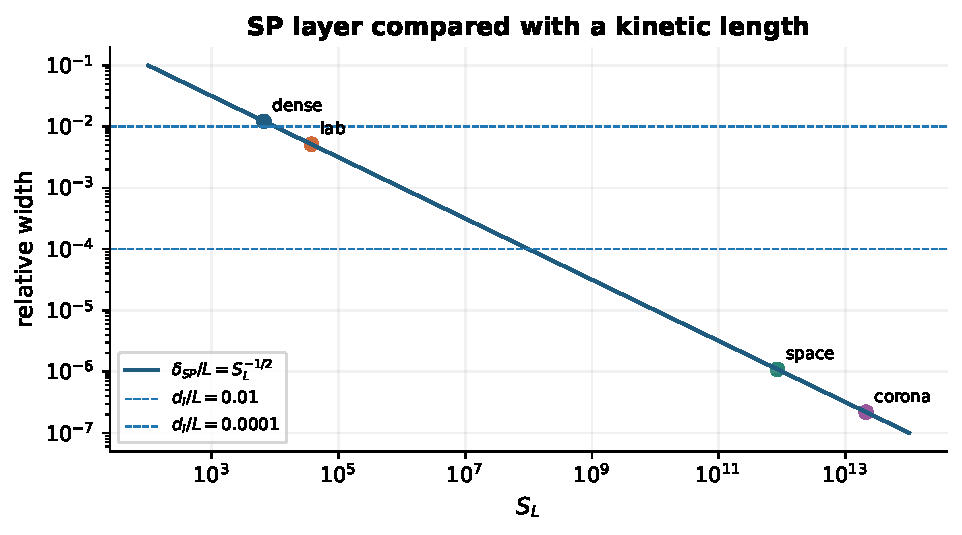
\includegraphics[width=.95\textwidth]{figures/07_sp.pdf}
\caption{Sweet--Parker层厚解析标度与固定$d_i/L$的比较。交点对应式\eqref{hall:spthreshold}；四个点来自教学参数。曲线不表示所有大$S$系统都能保持单一稳态长片。}\label{hall:figsp}\end{figure}

日冕教学例$L=10^7$ m、$V_A=3.4488\times10^6$ m/s给$S_L=2.10\times10^{13}$，经典层厚$2.182$ m，而$d_i=7.201$ m，比例$\delta_{SP}/d_i=0.303$。跨整个系统的Alfvén时间为2.90秒，按该单片SP入口速度处理系统磁通的时间为
\begin{equation}
\tau_{\rm SP}\sim\frac{L}{v_{\rm in}}=\tau_A\sqrt{S_L}
=1.33\times10^7\,\mathrm s\simeq154\,\text{天}.
\end{equation}
这个漫长时间只是该组输入与单片模型的结果，不是在模拟真实日冕事件。且$\lambda_{\rm mfp,e}\sim102$ km远大于2.18米，需要进一步核对粒子轨道和平行梯度的局地性，不能仅凭横向片厚判定碰撞闭合失效。实验室例与日冕例分别有$\nu_{ei}\tau_A=9.42$和168.5，它们也不是系统尺度上的完全无碰撞例。长片还可能先受撕裂不稳定性影响。应先改变模型或几何，不应把矛盾隐藏在一个调大电阻的参数里。

磁层教学例形式上给$\delta_{SP}=10.9$ m，甚至小于$\lambda_{De}=23.5$ m，也远小于$d_e=1680$ m。至此，使用准中性单流体经典SP层的多项排序一起失败；不能将这个数当作实际电子扩散区宽度。

\section{Hall层怎样改变流动，又为什么仍需要电子层}
在$d_e\ll\ell\lesssim d_i$的适用条件下，电子常仍保持近似磁化，而离子对局地电磁结构不能像大尺度那样即时响应。由于$\vct u_e=\vct u_i-\J/(en)$，磁通的运动可以接近电子流，离子质量通量的运动却与它不同。用一个共同速度和一个共同出口宽度的SP几何不再充分。

这种分离能够重排磁张力、面内电场、流入/排出通道及磁通输运，因而改变整体重联过程。但是取正压关系$p_e=p_e(n)$，并把电子电阻、惯性及非标量压力项删除后，
\begin{equation}
\E+\vct u_e\times\B=-\nabla h_e
\end{equation}
仍给出电子磁通冻结（若$h_e$是单值标量）。Hall项让磁场不再随\emph{离子}冻结，却未自动解除随\emph{电子}的冻结。有限电阻、非对角电子压力、电子惯性或明确的其他机制必须在电子内层中承担非理想作用。数值耗散也能做到，但必须诚实标明它是数值断线机制。\citep{Birn2001,Shay2001,Wang2015}

\section{为什么会出现四极面外磁场：用安培定律读图}
取二维$\partial_z=0$，面外场$B_z(x,y)$与面内电流满足
\begin{equation}
J_x=\frac{1}{\mu_0}\partial_yB_z,\qquad
J_y=-\frac{1}{\mu_0}\partial_xB_z.
\end{equation}
电子和离子的面内流不同，形成闭合的面内电流路径；这些电流会产生具有不同象限极性的$B_z$。反过来，测得二维$B_z$梯度可以推断面内电流。图\ref{hall:figquad}用一个显式解析函数检验此关系，既没有声称满足完整重联方程，也没有把电流线说成磁力线。
\begin{figure}[htbp]\centering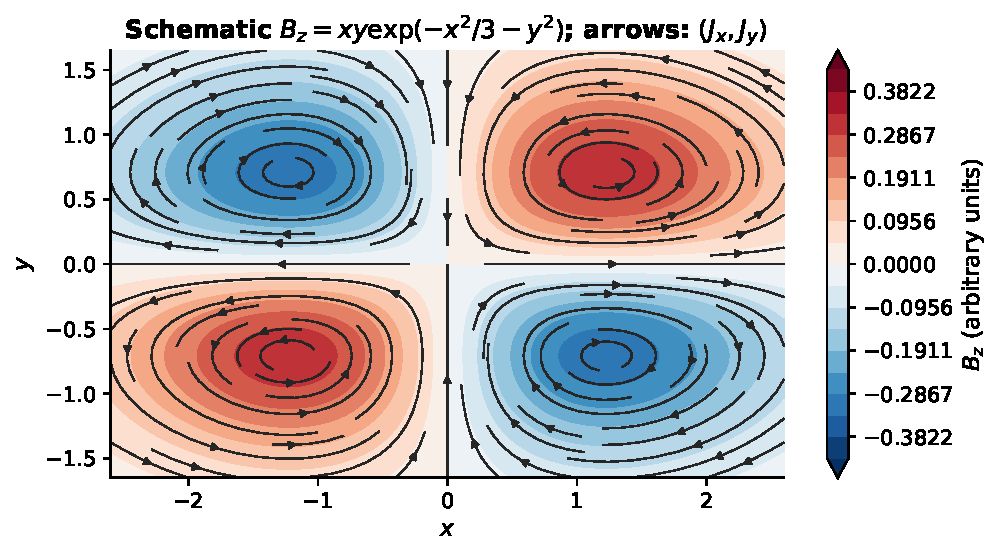
\includegraphics[width=.97\textwidth]{figures/05_quadrupole.pdf}
\caption{四极场与面内电流的教学示意。色彩是$B_z=xy\exp(-x^2/3-y^2)$，黑箭头严格由$J_x\propto\partial_yB_z,J_y\propto-\partial_xB_z$生成。颜色表示场的面外正负，箭头表示电流，二者不是同一种矢量。整体极性依反向场、坐标和电流方向改变。}\label{hall:figquad}\end{figure}

四极图样是重要线索，却不是“所有Hall预测已验证”的充分证据。导场、非对称、额外物种、三维结构和多个X点能使图样变形。要结合电子/离子流、电场分量和尺度判断。特别是反平行二维X点$\B=0$时，$\J\times\B=0$：\emph{旁边看到很强Hall场，并不能用它在零场X点直接支撑$E_z$。}

\section{重联率怎样从磁通计算}
在二维$A_z$约定下，$E_z=-\partial_tA_z$（取$\partial_z\phi=0$）。设X、O点位置都随时间变化，对磁通差作全导数：
\begin{align}
\frac{\dd}{\dd t}[A_z(O,t)-A_z(X,t)]
&=\partial_tA_z|_O+\dot{\vct x}_O\cdot\nabla A_z|_O
-\partial_tA_z|_X-\dot{\vct x}_X\cdot\nabla A_z|_X\\
&=E_z(X)-E_z(O).
\end{align}
第二步利用X和O都是$A_z$驻点，梯度为零。只有参考O点的$E_z$可忽略或已被适当扣除时，才将$E_z(X)$单独叫磁通变化率。归一率通常取$\mathcal R=E_{\rm rec}/(B_{\rm up}V_{A,\rm up})$；上游场、密度和位置要明确。若$B_{\rm up}$随时间改变，两个相同的归一率也可能对应不同的实际电压和功率。

\worked{速率不是功率，也不是温升}
取实验室例$B_{\rm up}=0.05$ T、$V_A=3.4488\times10^5$ m/s。若\emph{人为指定}某过程$\mathcal R=0.10$，则$E_{\rm rec}=1.7244\times10^3$ V/m。沿$z$长度0.2 m的均匀区，对应电动势约345 V。它只有与电流密度点乘、对体积积分后才成为功率；还需扣除边界Poynting通量、流能和热输运，才能讨论物种加热。这里的0.10是演示输入，不是由Hall方程独自推出来的普适常数。
